\chapter{Felhasználói dokumentáció}
\label{ch:user}
A LanDB (\textit{Language Database}) egy nyelvtanuló alkalmazás, amely japán és angol nyelvű szövegek automatikus feldolgozására és strukturált tárolására specializálódik. Az alkalmazás képes automatikusan felismerni a szövegekben szereplő szavakat, kifejezéseket és (japán nyelv esetén) kanji írásjeleket, majd ezekhez nehézségi szintet (CEFR, JLPT) és gyakorisági adatokat rendel. A felhasználó visszajelzései alapján a rendszer tudja követni a tudásszintet, és ismétlésre ajánlani a kevésbé ismert elemeket. A program fő célkitűzése a nyelvtanulók támogatása személyre szabott tanulási élmény nyújtásával. A projekt webes felületen keresztül érhető el, így a használatához csupán egy böngésző szükséges.

\section{Rendszerkövetelmények}

A projekt használatához az alábbi táblázatban látható minimális rendszerkövetelményeket kell figyelembe venni.

\begin{table}[H]
	\centering
	\begin{tabular}{ | m{0.25\textwidth} | m{0.65\textwidth} | }
		\hline
		\textbf{Komponens} & \textbf{Minimum / ajánlott verzió} \\
		\hline \hline
		\emph{Operációs rendszer} & Windows 10 / 11 \\
		\hline
        \emph{Internetkapcsolat} & Kezdeti telepítésekhez és angol fordítási funkciókhoz\\
		\hline
		\emph{Python} &  3.11 vagy újabb \\
		\hline
		\emph{Böngésző} & Google Chrome, Mozilla Firefox vagy Edge. \\
		\hline
        \emph{Memória} & Legalább 4 GB RAM \\
		\hline
        \emph{Tárhely} & Legalább 1 GB szabad hely (adatbázis és szótárak) \\
		\hline
	\end{tabular}
	\caption{Rendszerkövetelmények}
	\label{tab:example-1}
\end{table}

\section{Telepítés és első indítás}

A projekt használatához az alábbi lépéseket kell követni.

\begin{compactenum}
	\item\label{step:first} Töltsük le a teljes projektet (ZIP formában vagy GitHubról: https://github.com/balazspricz38/LanDB).
	\item Csomagoljuk ki egy tetszőleges mappába
	\item A lokális szerver elindításához dupla kattintással futtassuk a következő fájlt: \textit{start.bat}, vagy konzol segítségével a \textit{start.ps1} elnevezésű scriptet. Ezek automatikusan elvégzik a következő lépéseket:
    \begin{compactenum}
        \item Virtuális környezet létrehozása
        \item Függőségek telepítése a \textit{requirements.txt} fájlból
        \item Adatbázis inicializálása
        \item Nyelvi szótárak importálása
        \item A szerver elindítása \textit{http://127.0.0.1:8000/} címen\footnote{Ez a cím a program kész kiadása előtti kipróbálásához, teszteléséhez ajánlott.}
    \end{compactenum}
    \item Nyissuk meg a böngészőt és navigáljunk a \textit{http://127.0.0.1:8000} címre
\end{compactenum}

\section{A rendszer fő funkciói}

\subsection{Navigációs menü}

\begin{compactenum}
    \item \textbf{Home} - Kezdőlap, szövegfeldolgozás és feltöltés
    \item \textbf{Texts} - Feldolgozott szövegek böngészése
    \item \textbf{Words} - Szavak böngészése, kezelése
    \item \textbf{Kanji} - Japán írásjelek böngészése, kezelése
    \item \textbf{Dictionaries} - Szótárak listája, kezelése
\end{compactenum}

\subsection{Szövegelemzés és tokenizálás}

A rendszer lehetőséget biztosít különböző formátumú szövegek feltöltésére és feldolgozására. A feldolgozó modul a bemeneti szöveget automatikusan nyelvi elemekre bontja (mondatok, szavak, valamint japán nyelv esetén kanji írásjelek), majd eltárolja azokat a hozzájuk tartozó metaadatokkal együtt. Az elemzett tartalmak ezt követően különböző nézetekben (kártya, lista, statisztika) érhetők el, és további műveletek alapjául szolgálnak, például szótárak létrehozásához vagy tanulási folyamatokhoz.

\subsection{Nyelvi elemek böngészése és kezelése}

A \textit{Texts} menüpontban található az elemzett szövegek listája (lásd \ref{fig:text-list}.~ábra). A szövegekhez tartozó részletes oldalon a mondatok, szavak és japán nyelv esetén kanji írásjelek többféle nézetben (kártya, lista, statisztika) jelennek meg. A rendszer támogatja a szövegekhez kapcsolódó műveleteket, például szótár készítését, exportálást (Excel, CSV, Quizlet), valamint az elemek kezelését. A szöveg törlése esetén a kapcsolódó szavak az adatbázisban megmaradnak, így a tanulási statisztikák nem vesznek el.

\begin{figure}[H]
	\centering
	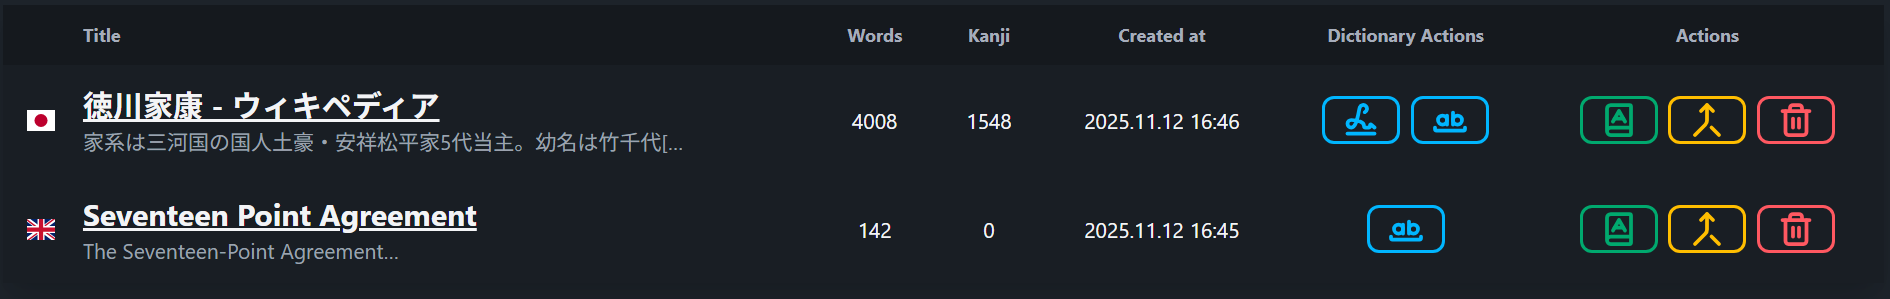
\includegraphics[width=1\textwidth]{images/user/text_list.png}
	\caption{Szövegek megjelenítése listában}
	\label{fig:text-list}
\end{figure}

A \textit{Words} és \textit{Kanji} menüpontokban a szavak és kanji írásjelek interaktív listanézetei érhetők el (lásd \ref{fig:kanji-list}.~ábra). A rendszer lehetőséget biztosít a nyelvi elemek szűrésére, keresésére és csoportos kezelésére. Az egyes elemekhez tartozó részletes oldalakon további információk, például olvasat, gyakoriság, tanulási előzmények és statisztikák jelennek meg. A rendszer támogatja a komponensek szótárakhoz rendelését és manuális hozzáadását is.

\begin{figure}[H]
	\centering
	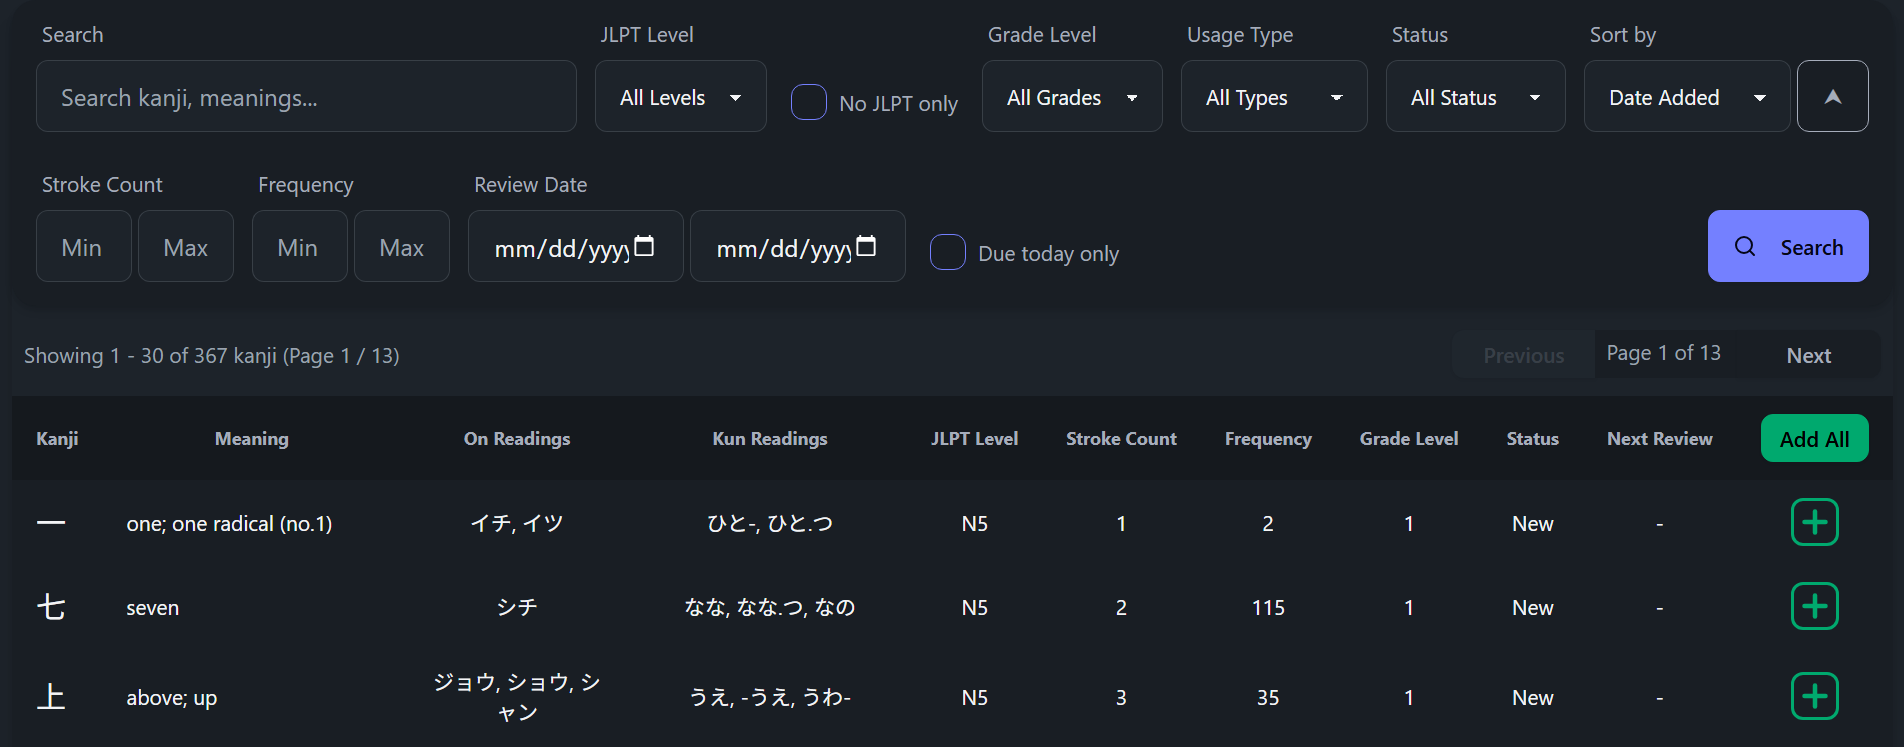
\includegraphics[width=1\textwidth]{images/user/kanji_list.png}
	\caption{Japán írásjelek listája és szűrői}
	\label{fig:kanji-list}
\end{figure}

\subsection{Szótárak kezelése és ismétléses tanulás}

A \textit{Dictionaries} menüpontban a felhasználó által létrehozott szótárak listája található. Egy szótár lehet szavakat vagy kanji írásjeleket tartalmazó gyűjtemény, amelyeket tetszőleges szövegből vagy akár manuálisan is létre lehet hozni. Az egyes elemekhez tartozó oldalon megtekinthetők a benne lévő nyelvi komponensek, statisztikák, valamint lehetőség van a beállítások módosítására, exportálásra vagy törlésre is. A szótárakhoz tartozó export funkciók lehetővé teszik, hogy a felhasználó saját tanulási anyagait más platformokon is felhasználhassa, vagy offline formában is elérje.

A rendszer támogatja az ismétlésen alapuló tanulást (spaced repetition), a szótárakban lévő szavak és kanji írásjelek tanulási státusza, következő ismétlésének ideje, valamint a felhasználó teljesítménye folyamatosan nyomon követhető. A tanulási felületen a program automatikusan kiválasztja a soron következő ismétlendő vagy új elemeket, és a felhasználó visszajelzései alapján frissíti a tudásszintet, illetve az ismétlési intervallumokat. Ezek a statisztikák valós időben frissülnek, így a tanuló azonnal láthatja a fejlődését és a hátralévő feladatokat. A program továbbá lehetőséget biztosít a szótárak közötti elemek kezelésére, valamint az adatok exportálására különböző formátumokba, támogatva a további feldolgozást és más tanulási rendszerekbe történő integrációt.

\begin{figure}[H]
	\centering
	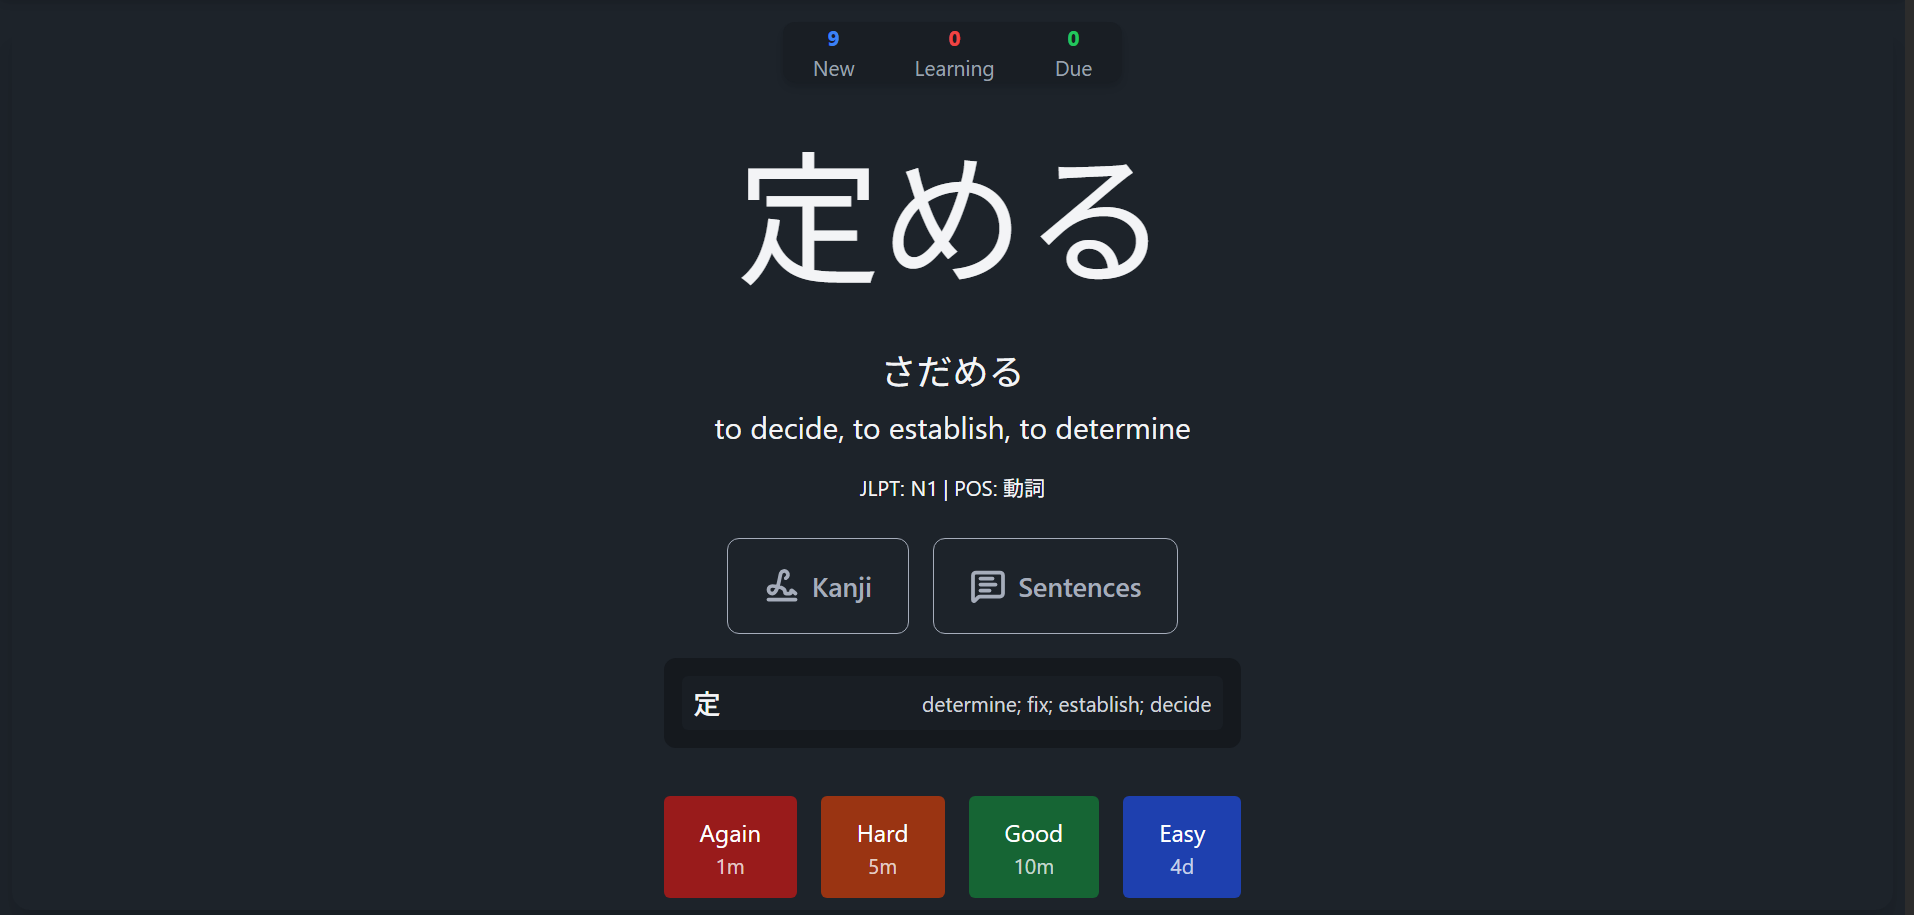
\includegraphics[width=1\textwidth]{images/user/srs_study.png}
	\caption{Japán írásjelek listája és szűrői}
	\label{fig:srs-study}
\end{figure}

\section{Használati útmutató}

Ebben a fejezetben, néhány gyakorlati példán keresztül mutatjuk be a LanDB rendszer használatát, szövegek elemezésétől kezdve a tanulásig.

\subsection{Japán szöveg elemzése kanji szótár létrehozásával}

Miután a \ref{fig:home-page}.~ábrán látható kezdőoldal betöltött, a felhasználó szöveget adhat meg elemzés céljából közvetlen bevitellel vagy fájl feltöltésével (\textit{.txt}, \textit{.docx}, \textit{.pdf}). A rendszer a bemeneti tartalmat validálja, majd nyelvi elemekre bontja, és elmenti a hozzá tartozó metaadatokkal együtt. Az elemzés után a felhasználó a feldolgozott szöveg oldalára kerül, ahol az eredmények különböző nézetekben (kártya, lista, statisztika) érhetők el, és az egyes elemek részletesen is megtekinthetők.

\begin{figure}[H]
	\centering
	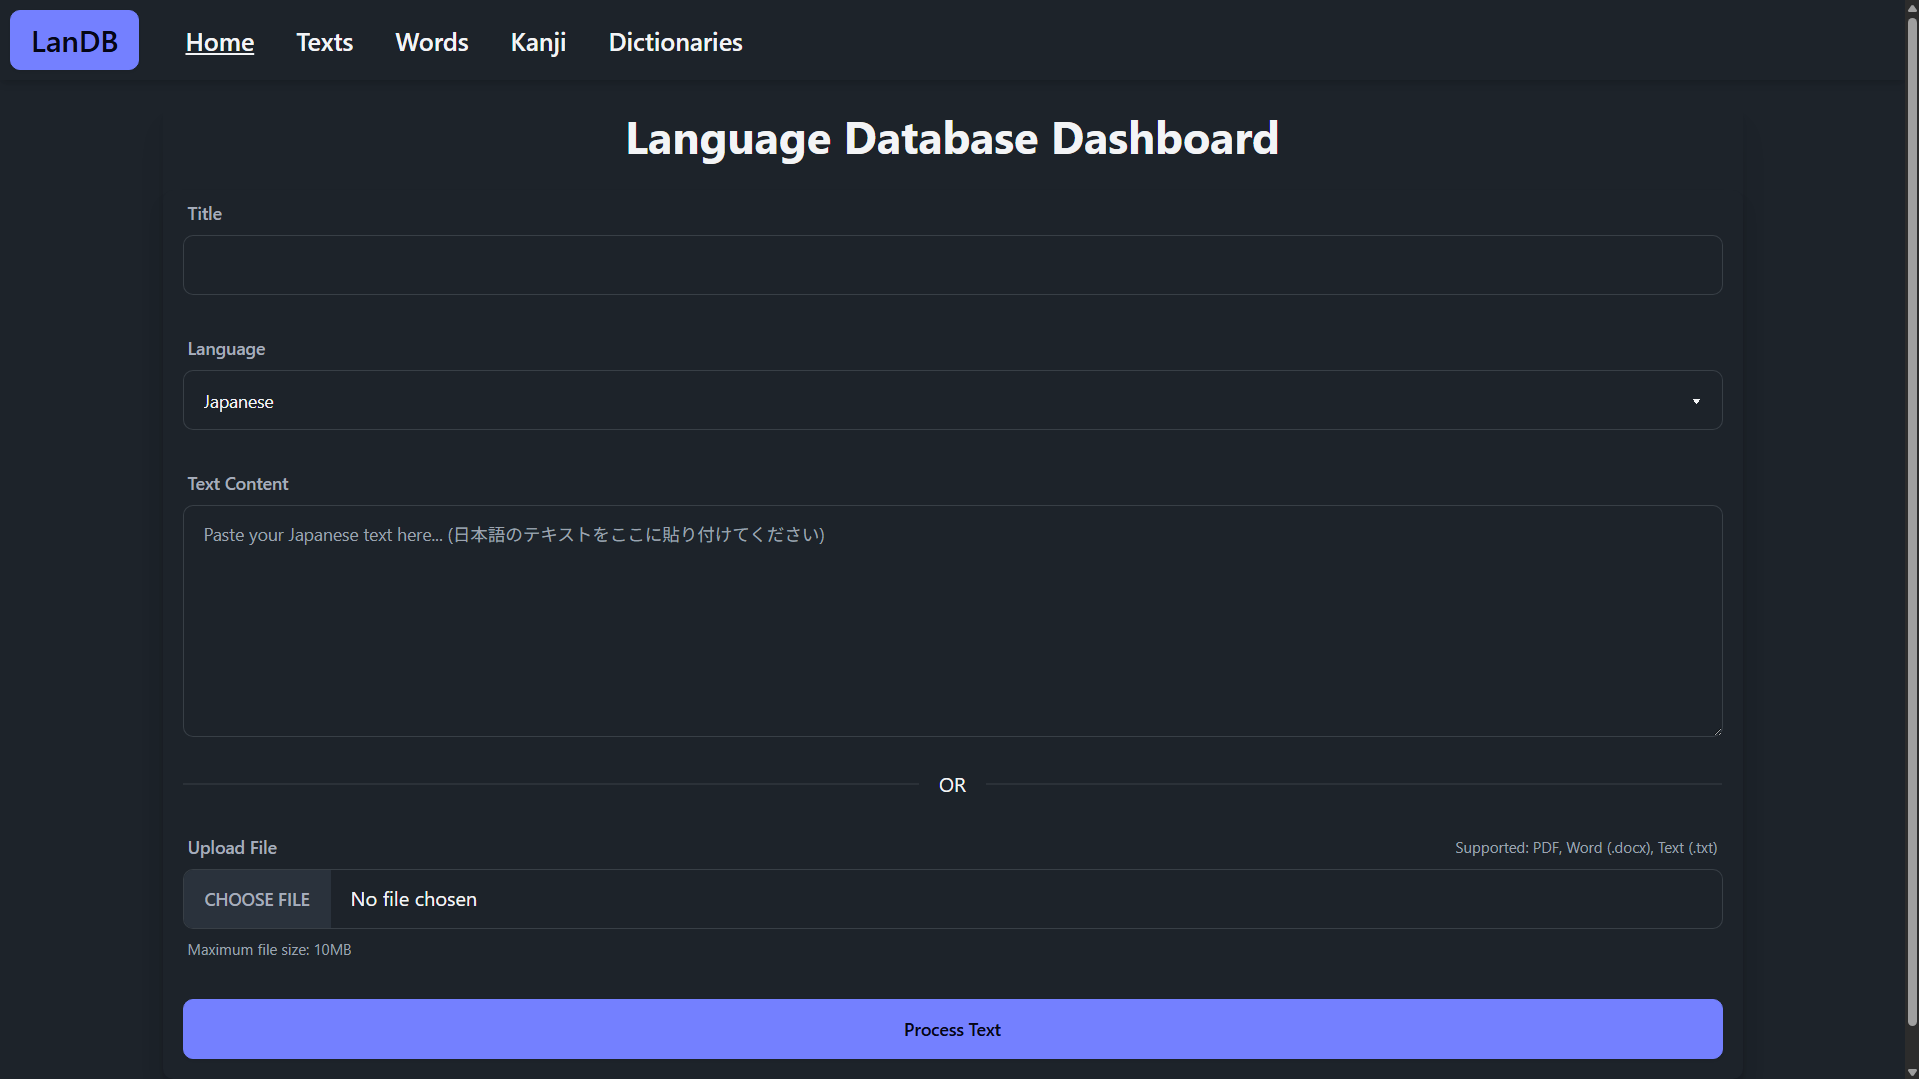
\includegraphics[width=1\textwidth]{images/user/home_page.png}
	\caption{Kezdőlap}
	\label{fig:home-page}
\end{figure}

\begin{enumerate}
    \item A főoldalon a \textit{New Text} gomb megnyomásával megadható a cím, kiválasztható a japán nyelv, majd beírható a szöveg vagy feltölthető egy fájl.
    \item A \textit{Process Text} gomb használatával a rendszer elvégzi az elemzést, és automatikusan a feldolgozott szöveg oldalára navigál. A megnyíló oldalon láthatók a mondatok, szavak és kanji írásjelek külön nézetekben.
    \item A \textit{Texts} menüpontban kiválasztható az elemzett szöveg, amelyből kanji szótár hozható létre.
    \item A megjelenő dialógusban nevet, és rövid leírást lehet adni az új szótárnak, de ezeket később is van lehetőség szerkeszteni. \ref{fig:create-kanji-dic}.~ábra:
    
    \begin{figure}[H]
	   \centering
	   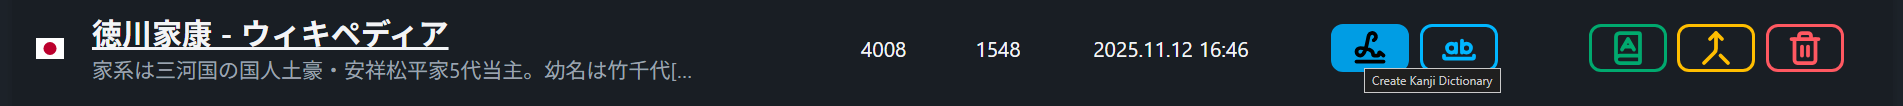
\includegraphics[width=1\textwidth]{images/user/create_kanji_dic.png}
	   \caption{Kanji szótár létrehozása}
	   \label{fig:create-kanji-dic}
    \end{figure}

    \item A \textit{Dictionaries} oldalon az új szótár megjelenik, amelynek nevére kattintva elindítható a tanulási folyamat.
    \item A kék információs gomb megnyomásával megtekinthetők a szótár elemei, amelyek eltávolíthatók, illetve a \ref{fig:dictionary-settings}.~ábrán látható szótárhoz tartozó beállítások is itt érhetőek el.
    
    \begin{figure}[H]
	   \centering
	   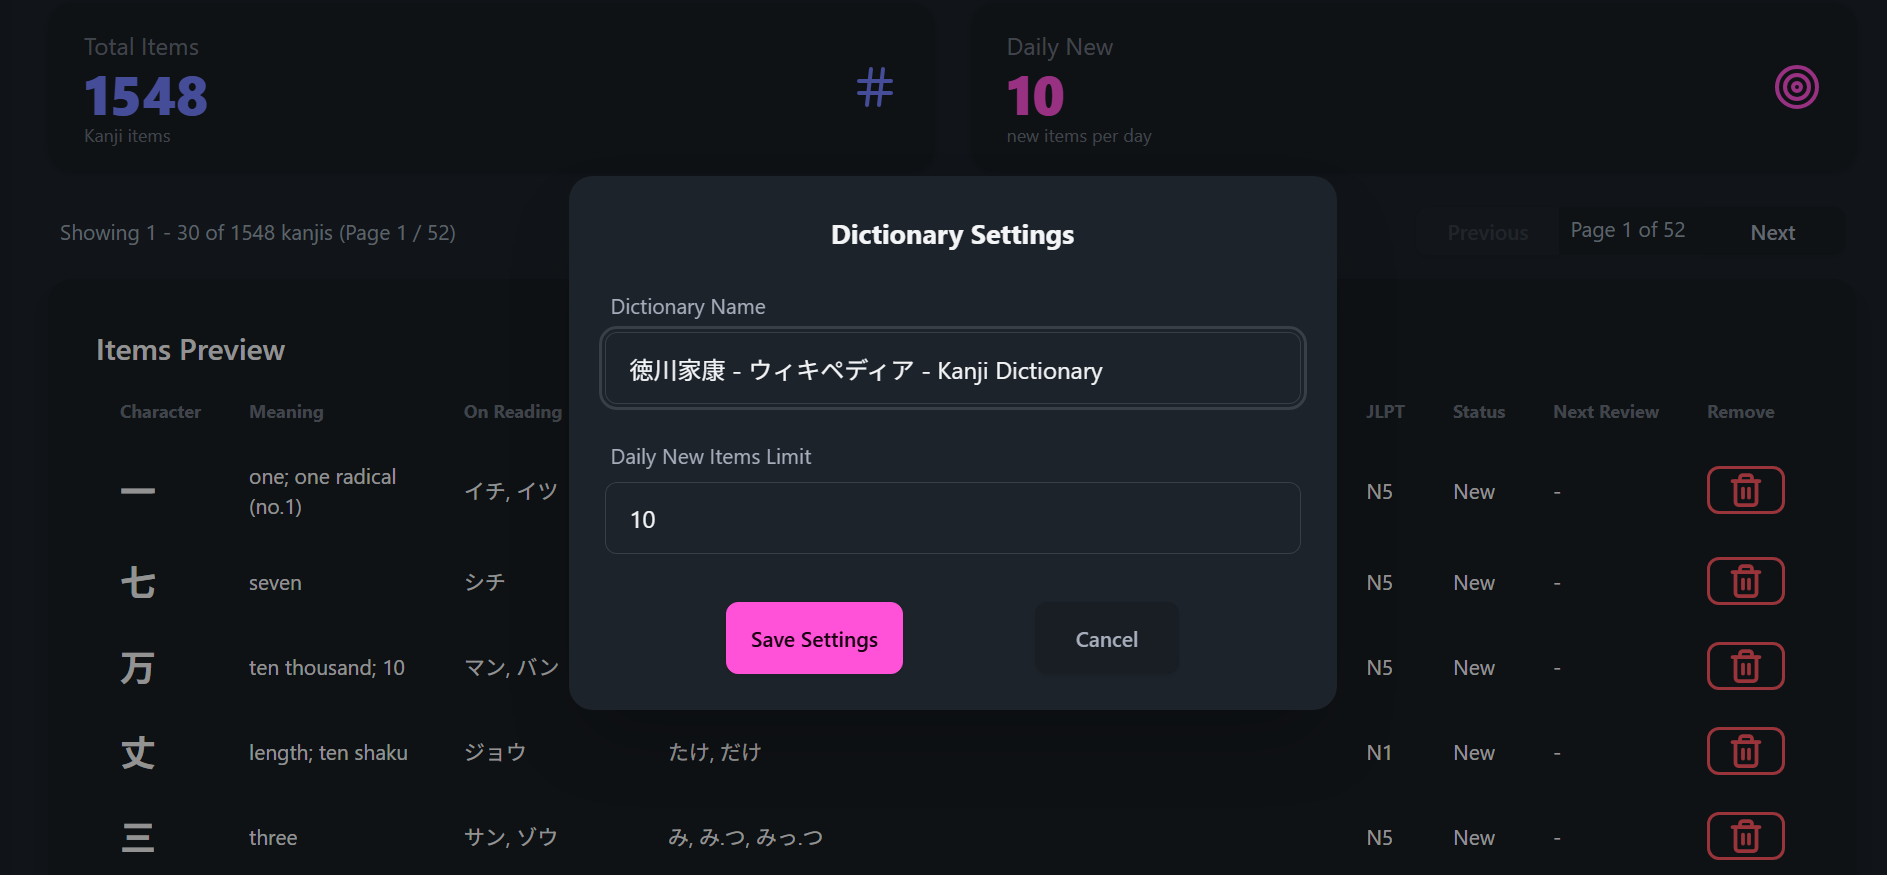
\includegraphics[width=1\textwidth]{images/user/dictionary_settings.png}
	   \caption{Szótár beállításai}
	   \label{fig:dictionary-settings}
    \end{figure}
\end{enumerate}

\subsection{Két angol szótár létrehozása és egyesítése}

\begin{enumerate}
    \item Az angol szöveg feltöltése és elemzése a korábban ismertetett módon történik.
    \item A \textit{Dictionaries} menüpontban két új angol szótár hozható létre, például egy az A1-es, egy másik az A2-es szavak számára.
    \item A \textit{Words} oldalon megjelenő listában először az angol szavakat kell kiválasztani, majd szűrni nyelvvizsgaszint és az őket tartalmazó szöveg szerint.
    \item A táblázat címsorában található \textit{Add All} gomb használatával az összes szűrt szó hozzáadható az új szótárhoz a  \ref{fig:filtered-to-dict}.~ábrán megjelenő ablakban.
    
    \begin{figure}[H]
	   \centering
	   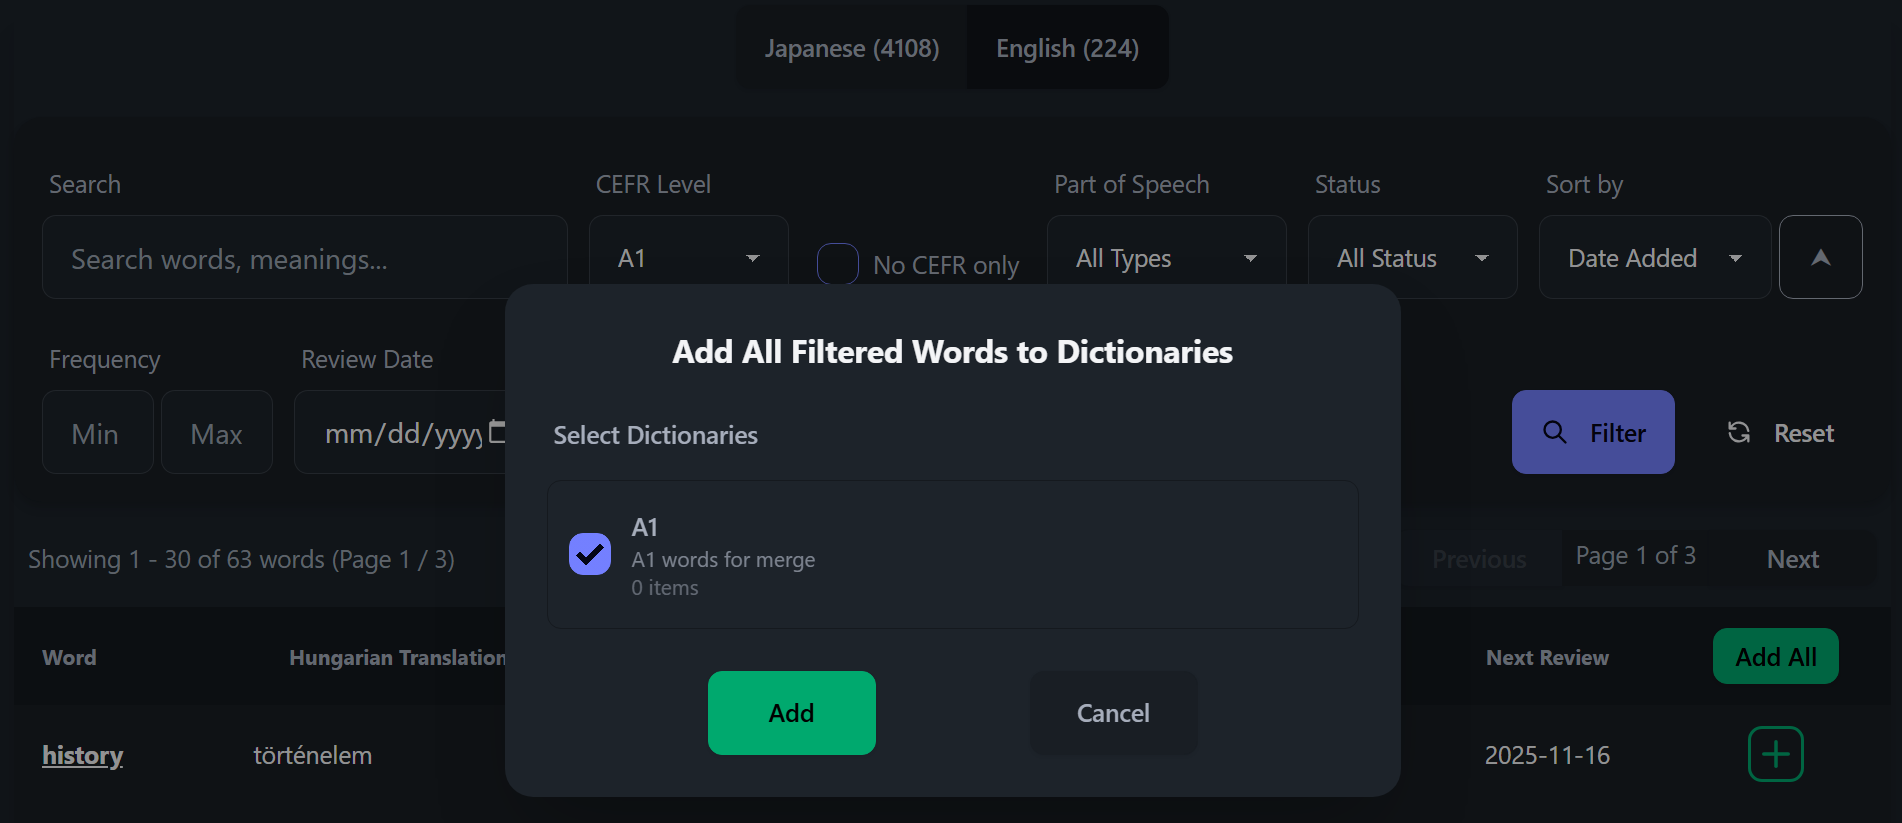
\includegraphics[width=1\textwidth]{images/user/filtered_to_dict.png}
	   \caption{A1 szavak hozzáadása szótárhoz}
	   \label{fig:filtered-to-dict}
    \end{figure}

    \item Az előző lépéshez hasonlóan az A2-es szavak is hozzáadhatók a másik szótárhoz, ezt követően a \textit{Dictionaries} oldalra lehet navigálni
    \item Az A1 listához tartozó narancssárga színű \textit{Merge} gomb megnyomásával csak a kiválasztott szótárral megegyező formátumú és nyelvű elemek válnak elérhetővé. A Merge gomb ismételt megnyomásával az egyesítés mód megszüntethető.
    \item A másik szótár kiválasztása után a \ref{fig:merge-dictionaries}.~ábrán látható felugró ablakban fejezhető be az egyesítési folyamat.

    \begin{figure}[H]
	   \centering
	   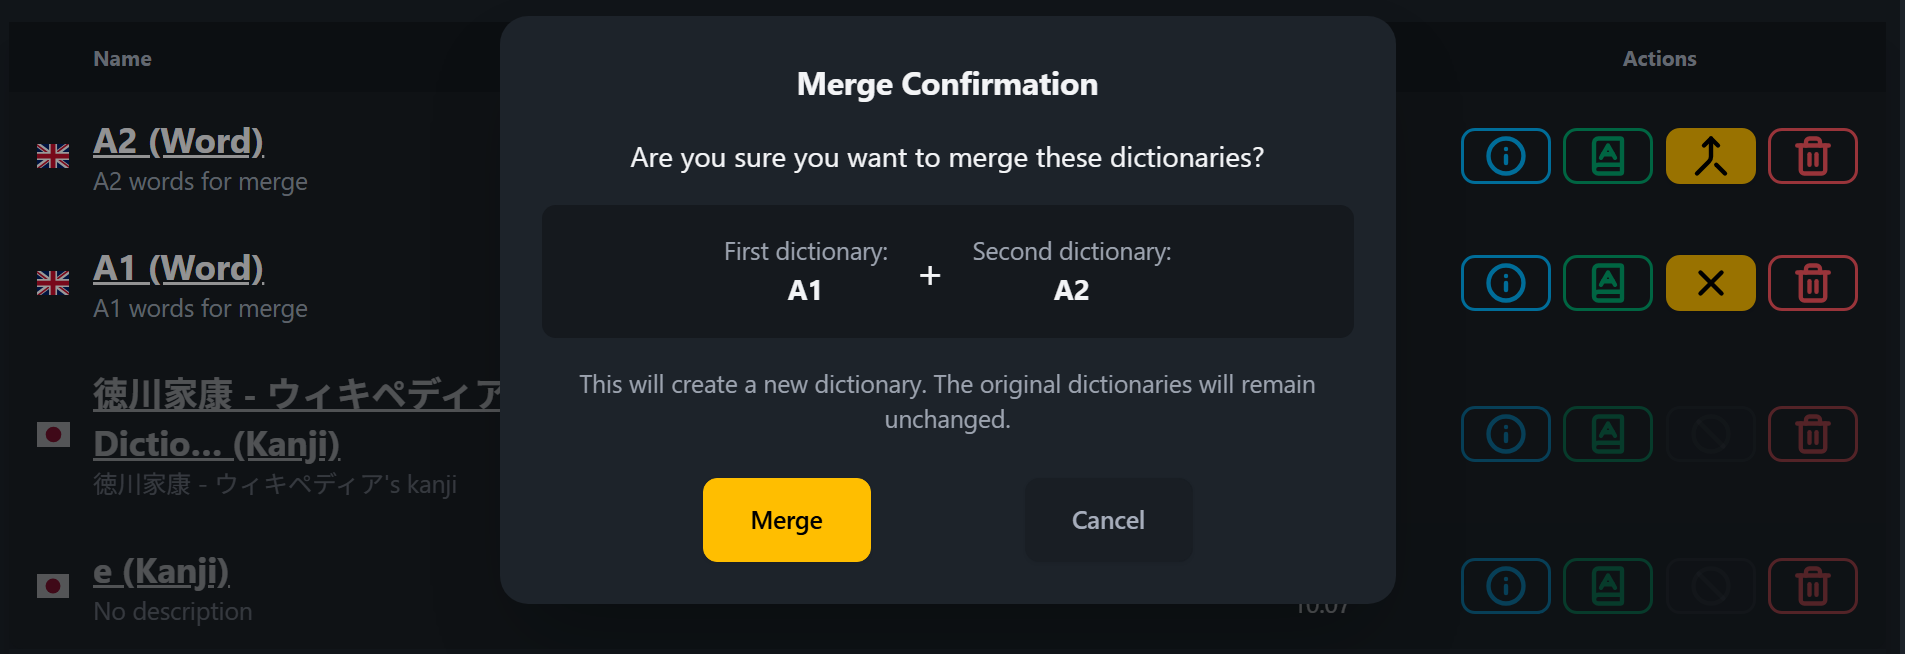
\includegraphics[width=1\textwidth]{images/user/merge_dictionaries.png}
	   \caption{A1 szótár hozzáadása az A2 szótárhoz}
	   \label{fig:merge-dictionaries}
    \end{figure}
    
    \item Ezek után, az új, A1-es és A2-es szavakat tartalmazó szótár láthatóvá válik, ahogy ezt a \ref{fig:successful-merge}.~ábrán megfigyelhetjük.

    \begin{figure}[H]
	   \centering
	   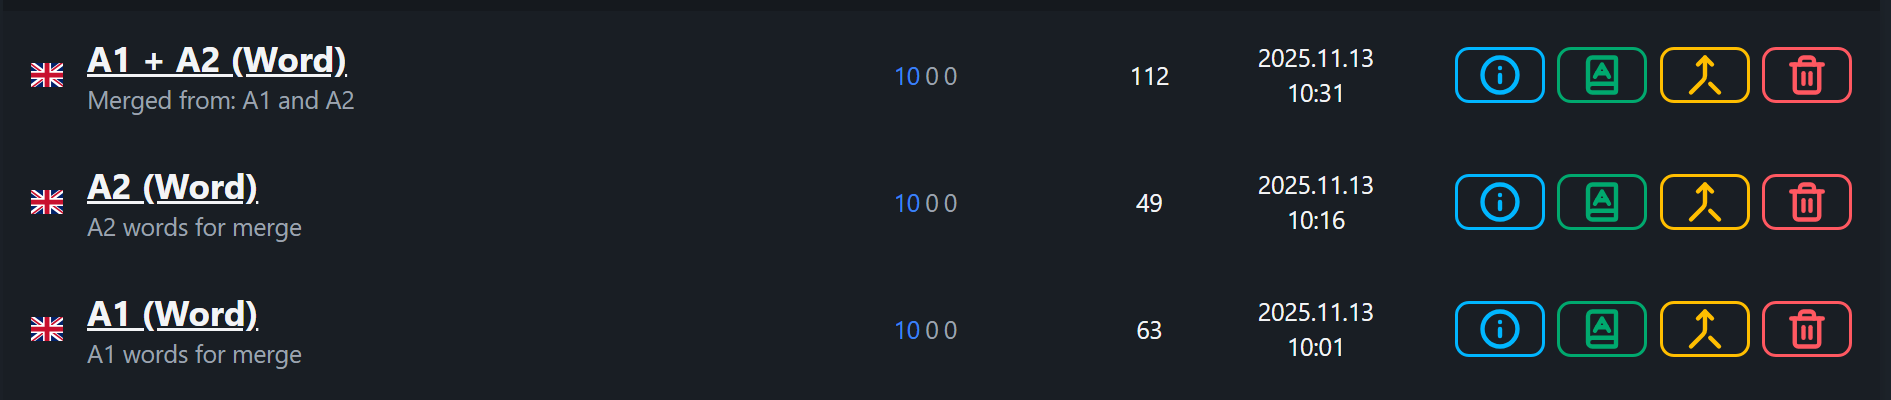
\includegraphics[width=1\textwidth]{images/user/successful_merge.png}
	   \caption{Az új szótár sikeresen létrejött}
	   \label{fig:successful-merge}
    \end{figure}
    
\end{enumerate}

\subsection{Ismétléses tanulás folyamata}

\begin{enumerate}
    \item A tanulni kívánt szótár kiválasztása után elindítható a tanulási folyamat.
    \item A rendszer automatikusan kiválasztja azokat a szavakat vagy kanji írásjeleket, amelyeket ismételni szükséges, valamint az új, eddig nem tanult elemeket.
    \item Az ismétlendő és új elemek száma a szótár információs oldalán módosítható, azonban a rendszer alapértelmezés szerint napi 10 új kifejezés tanulását engedélyezi.
    \item Egy elemnek először csak az idegen nyelvű olvasata jelenik meg, a "kártyát" a \textit{Show Answer} gomb megnyomásával lehet megfordítani.
    \item Megfordítás után van lehetőség a szóhoz kapcsolódó mondatok és írésjelek megjelenítésére (ha léteznek), valamint kanji írásjeleknél az őt tartalmazó szavakéra. Továbbá itt található a négy, tudásszint alapján választható gomb. Ezek alapján ad a tanuló visszajelzést, hogy milyen mértékben tudta, ismerte fel a kifejezést.
    \item A rendszer minden válasz után frissíti az adott elem tanulási státuszát, és ennek megfelelően ütemezi a következő ismétlés időpontját.
    \item Ha a napi ismétlések és új elemek száma eléri a nullát, az aznapi tanulási folyamat véget ért. Ekkor természetesen van lehetőség az új elemek megengedett felső korlátját növelni, ilyenkor folytatódhat a folyamat. 
\end{enumerate}

\section{Hibakezelés és gyakori problémák}

A rendszer a legtöbb felhasználói hibát közvetlenül a felületen, jól látható hibaüzenettel jelzi. Az alábbiakban összefoglaljuk a leggyakoribb hibákat és azok kezelését:

\begin{description}
	\item[Kötelező mezők hiánya] Szöveg feltöltésekor nincs megadott cím. Ha ez hiányzik, a rendszer figyelmeztető üzenetet jelenít meg, és nem engedi a feldolgozást.
	\item[Érvénytelen vagy üres fájl feltöltése] Ha a feltöltött fájl nem tartalmaz szöveget vagy az adott nyelv felismeréséhez szükséges karaktereket, a rendszer hibaüzenetet ad vissza.
    \item[Érvénytelen vagy üres szöveg megadása] Az fent említett esethez hasonlóan ellenőrzés után hibaüzenet látható.
    \item[Egyszerre fájl és szöveg megadás] A program a szöveges adatokat részesíti előnyben, a feltöltött fájl ilyenkor nem kerül feldolgozásra.
	\item[Szótárak létrehozásakor hiányzó adatok] Új szótár létrehozásánál kötelező megadni a nevet, a nyelvet és a tartalom típusát (szó vagy kanji). Ha valamelyik hiányzik, a rendszer nem hozza létre a szótárat, és hibaüzenetet jelenít meg.
    \item[Szótárak összevonása] Nem lehet ugyanazt a szótárat önmagával összevonni, illetve csak azonos típusú szótárak vonhatók össze. Bár a program a felhasználónak közvetlenül nem engedélyezi ezek összevonását, a nem megfelelő paraméterű elemeket nem elérhetővé teszi, de ha ennek ellenére rossz hívást kapna a szerver, figyelmeztető üzenet jelenik meg.
    \item[Exportálásnál hiányzó választás] Ha exportáláskor nem választott formátumot vagy típust meg a felhasználó, a rendszer hibaüzenetet jelenít meg.
    \item[Ismeretlen oldal, vagy objektum] Ha a felhasználó nem létező objektumhoz tartozó oldalra vagy nem létező címre navigálna, egyedi \texttt{404 error} oldalról vissza tud térni a kezdőlapra.

\section{Adatkezelés és Biztonság}

A rendszer minden adatot helyileg tárol, ehhez külső felhőszolgáltatásokat vagy hálózati adatbázisokat nem vesz igénybe. Az alkalmazás alapértelmezett adatbázisa a projekt gyökérkönyvtárában található, és a nyelvi elemek, szövegek, tokenek, valamint szótárbejegyzések tárolására szolgál. A japán nyelvhez kapcsolódó segédadatok CSV formátumban, szintén lokálisan kerülnek tárolásra, így az alkalmazás ezen részének működéséhez nincs szükség külső szerverkapcsolatra. Az angol szavak automatikus fordításához a \texttt{Deep Translate} csomagot használja, amely internetes kapcsolaton keresztül működik.

Az exportálási és importálási funkciók kizárólag a felhasználó saját környezetében futnak. Ezek a fájlok nem kerülnek a projektben belül mentésre, az exportálások eredményét a böngészőn keresztül van lehetőség letölteni.

Mivel a jelenlegi verzióban nincs külön felhasználókezelés, az alkalmazás közös adatbázist használ, ezért több felhasználó esetén ugyanazok az adatok lesznek elérhetők. Ennek biztonsági kockázatát a rendszer lokális futtatási környezete csökkenti, azonban a jövőbeli fejlesztési tervek között szerepel a felhasználói fiókok és jogosultságkezelés bevezetése az adatbiztonság növelése érdekében.

\end{description}